%%%%%%%%%%%%%%%%%%%%%%%%%%%%%%%%%%%%%%%%%%%%%%%%%%%%%%%%%
%                                                       %
%  	     PRESENTACIÓN - TRABAJO DE FIN DE MASTER		%
% 														%
%					UNAI ALDASORO MARCELLAN             %
%%%%%%%%%%%%%%%%%%%%%%%%%%%%%%%%%%%%%%%%%%%%%%%%%%%%%%%%%


%%%%%%%%%%%%%%%%%%%%%%%%%%%%%%%%%%%%%%%%%%%%%%%%%%%%%%%%%%%%%%%%%
%                                                         		%
%  TEMA PRINCIPAL Y CONFIGURACIÓN DE COLORES BASADOS EN:  		%
% 														  		%
%					beamerthemeDigna.sty						%
%																%
% Copyright 2007 by Till Tantau									%
% Modified by Digna Gonzalez based on beamer 					%
% theme Diuf (by Till Tantau) and Tornio (by Marco Barisione)	%
%																%
%%%%%%%%%%%%%%%%%%%%%%%%%%%%%%%%%%%%%%%%%%%%%%%%%%%%%%%%%%%%%%%%%

% TIPO DE DOCUMENTO
\documentclass[xcolor=dvipsnames, utf8, spanish]{beamer} %[xcolor=dvipsnames]
% para poder utilizar mas colores estandares

% PAQUETES A UTILIZAR
% \usepackage[utf8]{inputenc}
% \usepackage[spanish]{babel}
\usepackage{amsthm}
\usepackage{booktabs}
\usepackage{graphicx} %para poder trabajar con graficos
\usepackage{colortbl}
\usepackage{yhmath} %para poder utilizar el simbolo de numero periodico
\usepackage{etex}
\usepackage[all]{xy}

% TEMA PRINCIPAL Y CONFIGURACIÓN DE COLORES
\usetheme{Digna}
\usecolortheme[RGB={199, 21, 133}]{structure}
\usecolortheme{freewilly}

% INFORMACION GENERAL DEL DOCUMENTO
\title [Problema multimercado de oferta óptima]{OPTIMIZACIÓN DE MODELOS ESTOCÁSTICOS DE MERCADO ELÉCTRICO MÚLTIPLE MEDIANTE MÉTODOS DUALES}
\author[Unai Aldasoro Marcellan]{Unai Aldasoro Marcellan}
\institute{TFM - MIEIO curso 2010/2011}


% INICIO DEL DOCUMENTO
\begin{document}
\newenvironment{specialframe}{\begin{frame}[fragile,environment=specialframe]}{\end{frame}}

% Insertar indice al cambiar de seccion
\AtBeginSection[]
	{\begin{frame}
		\frametitle{Índice}
		\scriptsize
		\tableofcontents[currentsection]
	\end{frame}}


% Portada
\begin{frame}[plain]
	\titlepage
	\begin{center}
		Director: Francisco Javier Heredia Cervera \\
		\textbf{programación estocástica, optimización dual, mercados eléctricos}
	\end{center}
\end{frame}


% Contenido principal

\section{Introducción}

\begin{frame}
	\frametitle{Contexto de investigación}
	\begin{exampleblock} {Proyecto de investigación DPI2008-02153. MCI}
		Short and Medium-Term multimarket Optimal Electricity Generation Planning with Risk and Environmental Constraints
	\end{exampleblock}
	\bigskip  
	\textbf{ENTORNO ACADÉMICO}
	\begin{itemize}
		\item Group on Numerical Optimization and Modeling (GNOM)
	\end{itemize}
	\bigskip
	\textbf{ENTE PROMOTOR OBSERVADOR}
	\begin{itemize}
		\item Gas Natural - Unión Fenosa
	\end{itemize}
\end{frame}


\begin{frame}
	\frametitle{Objetivos}
	\begin{exampleblock} {Objetivo principal}
		Valorar posibles métodos duales y contruir la base de una resolución eficiente del modelo eléctrico multimercado de oferta óptima en el MIBEL
	\end{exampleblock}
	\bigskip
	Modelo de optimizazión basado en \textbf{``Optimal Day-Ahead Bidding in the MIBEL's Multimarket Energy Production System''} C. Corchero and F.J Heredia
\end{frame}


\begin{frame}
	\frametitle{Descripción del problema: MIBEL}
	\begin{center}
		\xymatrix@R=0.5cm @C=1.2cm{
			&*+[F]\txt{Compañía\\generadora} \ar[r]^{oferta}
			&

\includegraphics[width=0.2\linewidth]{figuras/MIBEL_ZOOM.JPG} \ar[d]
			&*+[F]\txt{Compañía\\distribuidora} \ar[l]_{demanda} \\
			&*{} &*+[F] \txt{\scriptsize \em Precio de mercado} &  *{}
		}
	\end{center}
\end{frame}


\begin{frame}
	\frametitle{Descripción del problema: Estructura del mercado}
	\begin{columns}
		\begin{column} {.45\textwidth}
			\structure{Mercados MIBEL}
			\begin{itemize}
				\item Day-Ahead Market (DAM)
				\item Reserve Market (RM)
				\item Intraday Market (IM)
			\end{itemize}
			\bigskip
			\structure{Generación no optimizable}
			\begin{itemize}
				\item Bilateral Contracts (BC)
				\item Furures Contracts (FC)
			\end{itemize}
		\end{column}

		\begin{column} {.4\textwidth}
			\begin{figure}
			
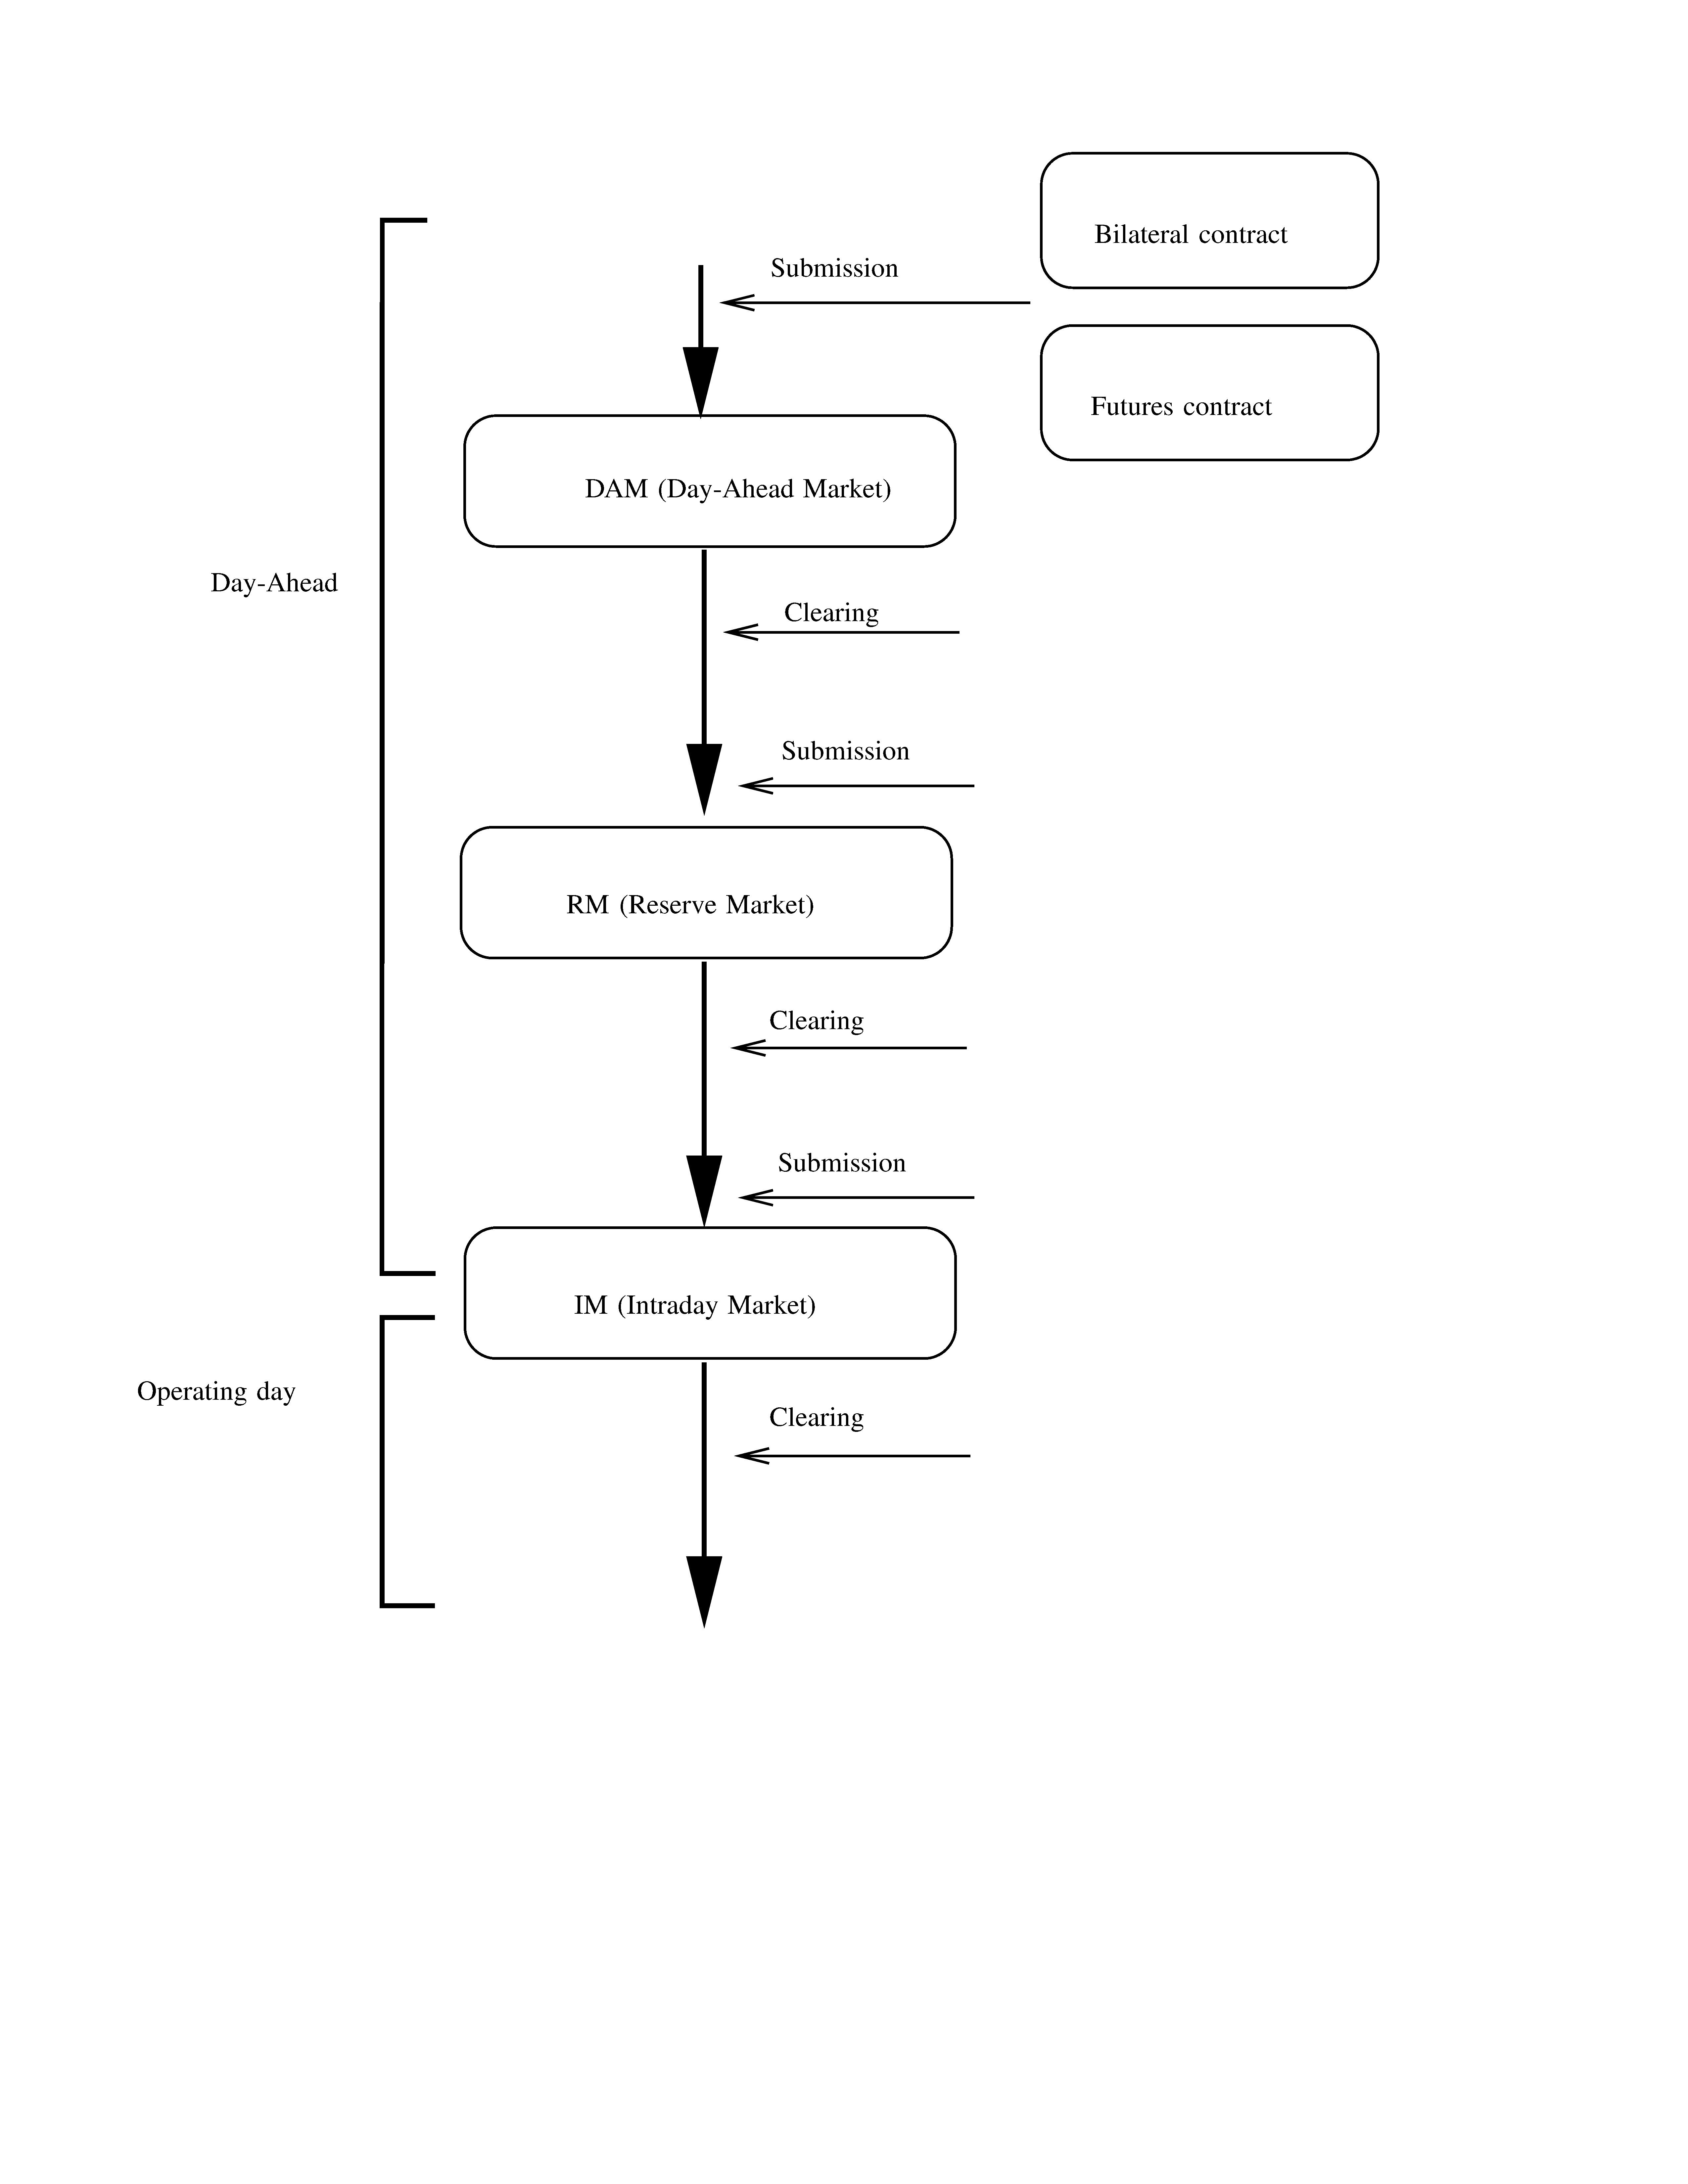
\includegraphics[width=1.2\linewidth]{figuras/esquemaMercados.JPG}
		\end{figure}
		\end{column}
	\end{columns}
\end{frame}



\begin{frame}
	\frametitle{Descripción del problema: Incertidumbre}
	\begin{center}
		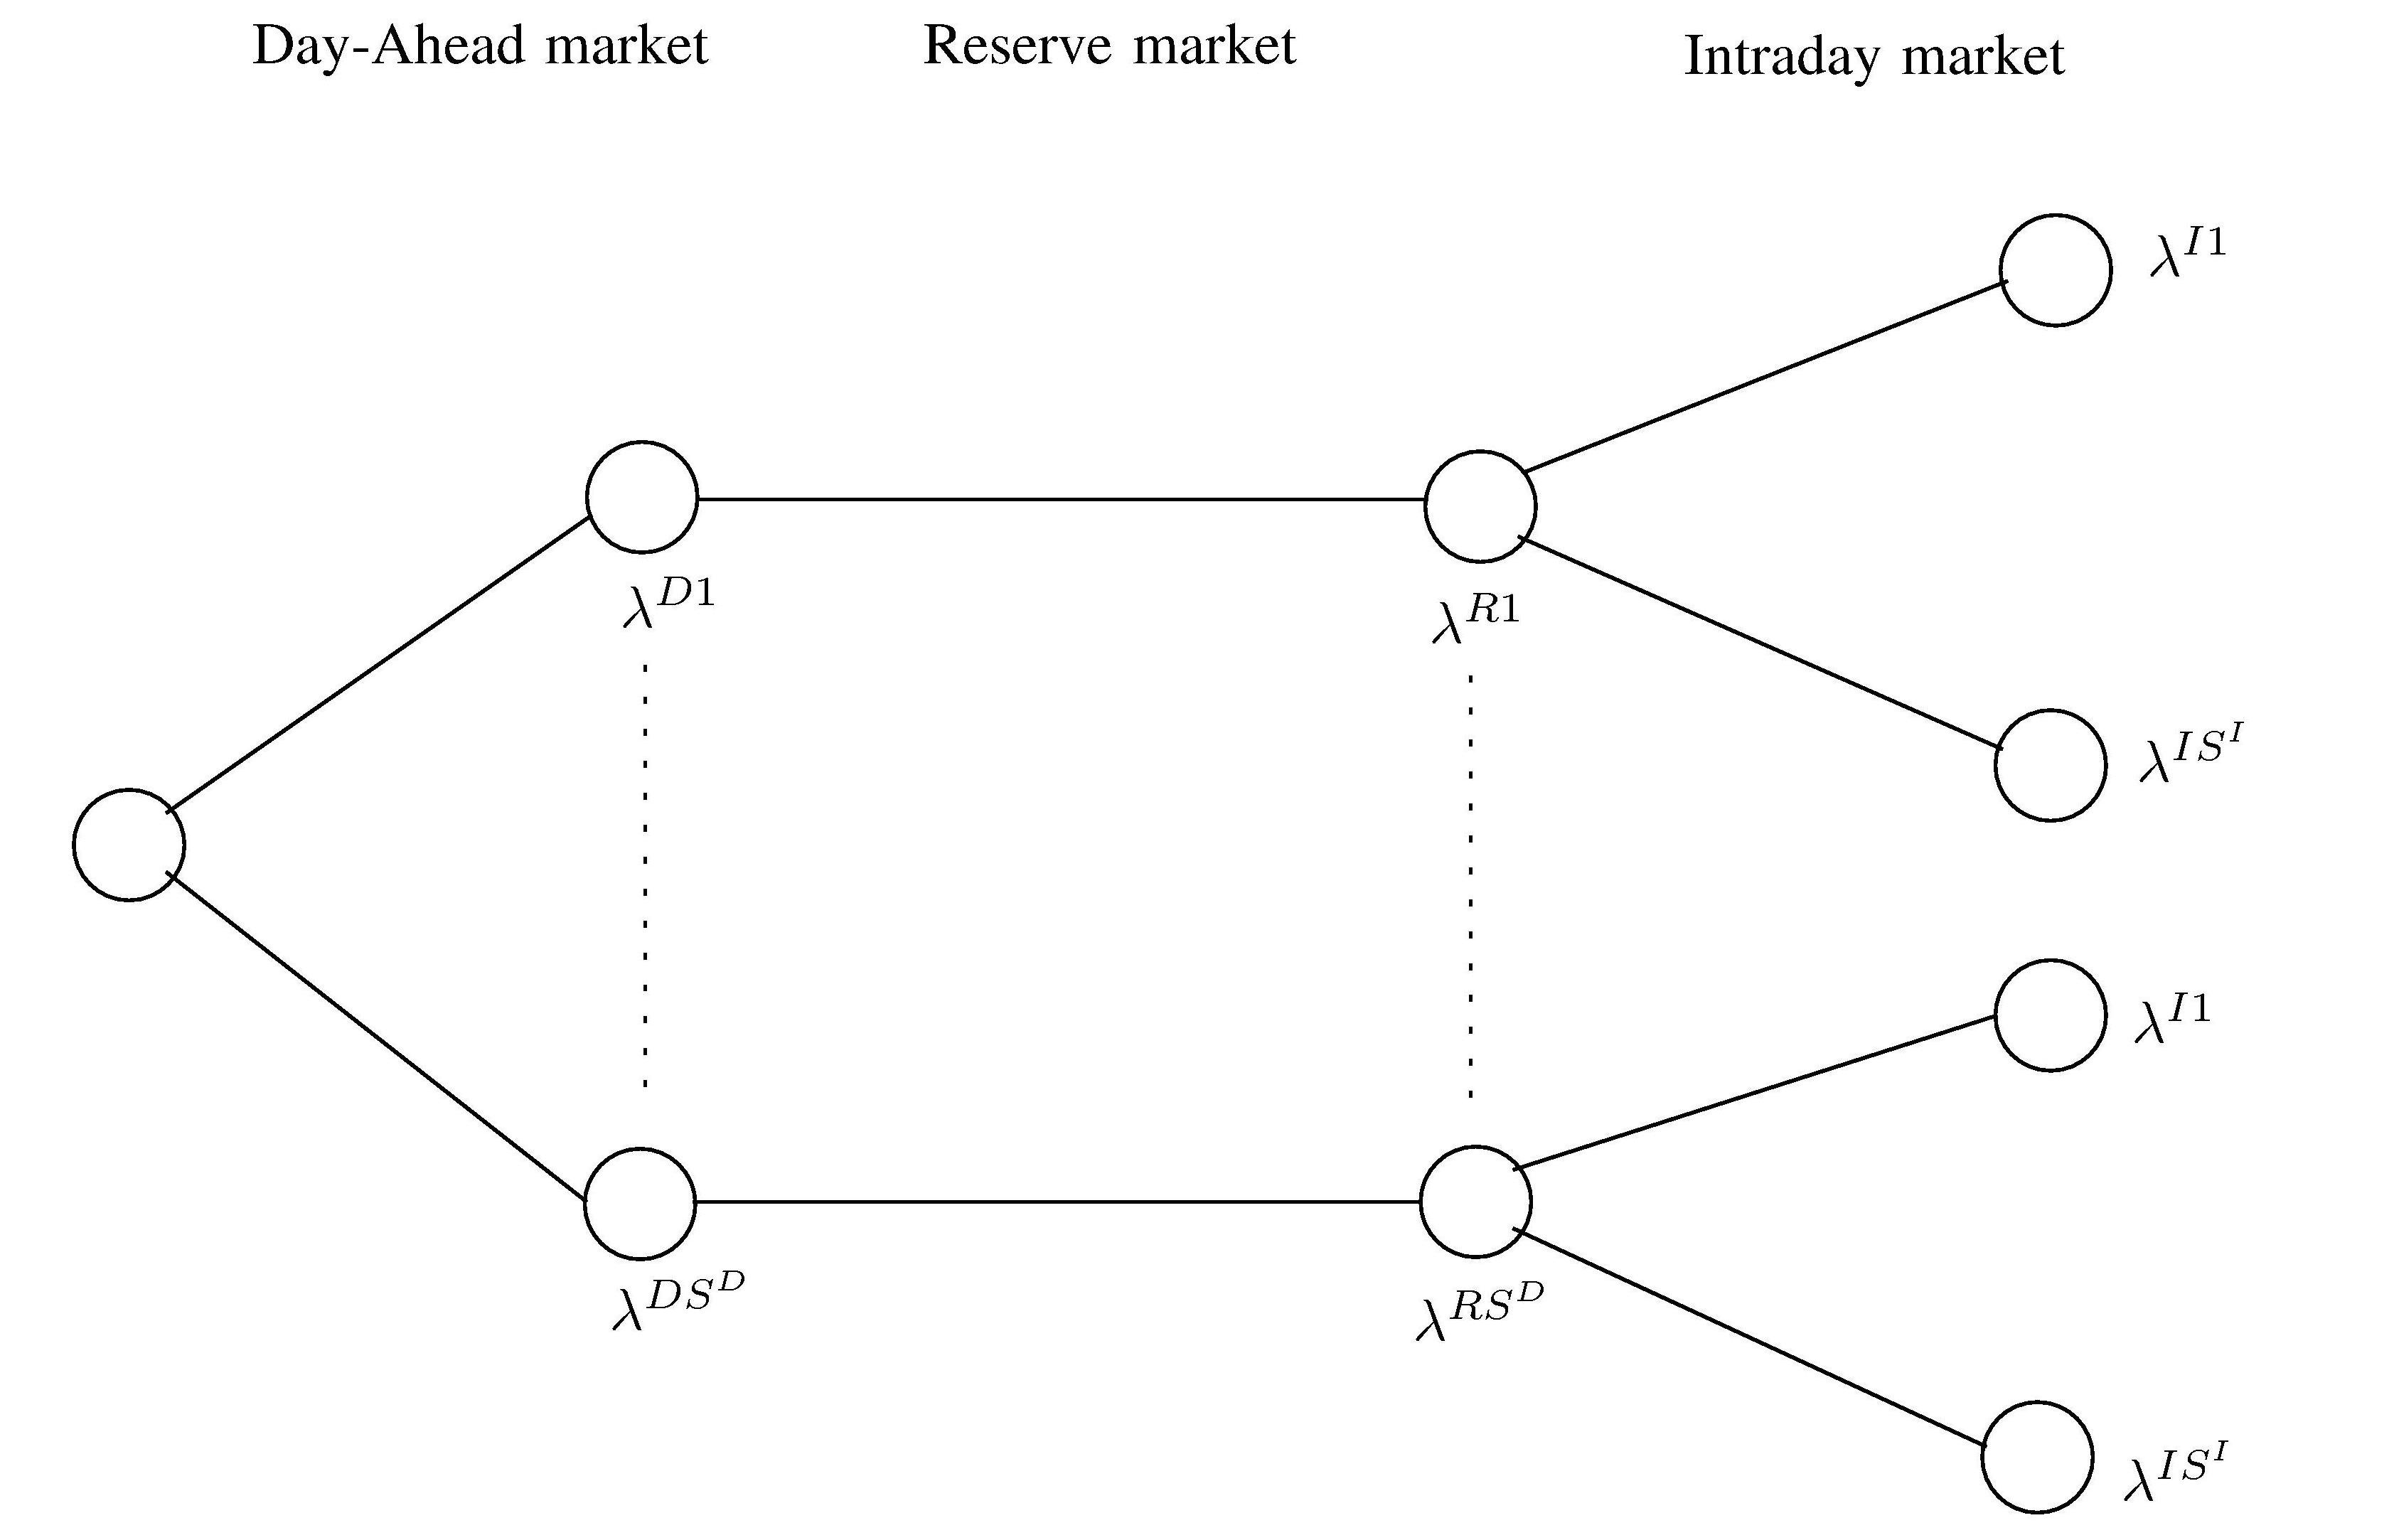
\includegraphics[width=8cm]{figuras/zuhaitza.jpg}
	\end{center}
\end{frame}


\begin{frame}
	\frametitle{Hipótesis}
	\begin{exampleblock} {Hipótesis 1}
		Sólo se decidirá si una unidad participa o no en IM.
	\end{exampleblock}
	\bigskip 
	\begin{exampleblock} {Hipótesis 2}
		Se considera únicamente la primera sesión de IM.
	\end{exampleblock}
	\bigskip 
	\begin{exampleblock} {Hipótesis 3}
		Todas las pujas realizadas en los RM e IM serán casadas.
	\end{exampleblock}
\end{frame}



\section{Modelo de optimización}

\subsection{Conjuntos y elementos}

\begin{frame}
	\frametitle{Conjuntos y elementos}
	\begin{block} {Conjuntos y elementos}
		\begin{itemize}
			\item [$U_{j}$] Conjunto de unidades cuya generación es asignable (parcial o totalmente) a la demanda del contrato j de tipo FC
		\end{itemize}
		\begin{columns}
			\begin{column} {.5\textwidth}
				\begin{itemize}
				\item [$T$] Conjunto de \textbf{intervalos}
				\item [$I$] Conjunto de \textbf{unidades}
				\item [$S$] Conjunto de \textbf{escenarios}
				\item [$F$] Conjunto de \textbf{contratos FC}
				\item [$B$] Conjunto de \textbf{contratos BC}
				\end{itemize}
			\end{column}
			\begin{column} {.5\textwidth}
				\begin{itemize}
				\item [$t$] Elemento del conjunto T
				\item [$i$] Elemento del conjunto I
				\item [$s$] Elemento del conjunto S
				\item [$j$] Elemento del conjunto F
				\item [$bc$] Elemento del conjunto B
				\end{itemize}
			\end{column}
		\end{columns}
	\end{block}
\end{frame}

\subsection{Constantes}

\begin{frame}
	\frametitle{Constantes}
	\begin{block} {Caracterización de la incertidumbre}
		\begin{itemize}
			\item [$P^s$] \textbf{Probabilidad} del escenario s
			\item [$\lambda^{D,s}_t$] \textbf{Precio} de mercado \textbf{DAM} en el intervalo t bajo el escenario s
			\item [$\lambda^{R,s}_t$] \textbf{Precio} de mercado \textbf{RM} en el intervalo t bajo el escenario s
			\item [$\lambda^{I,s}_t$] \textbf{Precio} de mercado \textbf{IM} en el intervalo t bajo el escenario s
		\end{itemize}
	\end{block}
\end{frame}


\begin{frame}
	\frametitle{Constantes}
	\begin{block} {Coeficientes de coste}
		\begin{itemize}
			\item [$c^{b}_i$] Coeficiente de coste de \textbf{funcionamiento} de la unidad i
			\item [$c^{on}_i$] Coeficiente de coste de \textbf{encendido} de la unidad i
			\item [$c^{off}_i$] Coeficiente de coste de \textbf{apagado} de la unidad i
			\item [$c^{l}_i$] Coeficiente de coste \textbf{lineal} de la unidad i
			\item [$c^{q}_i$] Coeficiente de coste \textbf{cuadrático} de la unidad i
		\end{itemize}
	\end{block}
\end{frame}



\begin{frame}
	\frametitle{Constantes}
	\begin{block} {Constantes de generación}
		\begin{itemize}
			\item [$g_i$] Capacidad de generación ACG de la unidad i
			\item [$\overline{P}_i$] Máxima capacidad de generación de la unidad i
			\item [$\underline{P}_i$] Mínima capacidad de generación de la unidad i
			\item [$R_i$] Cota superior de la diferencia de generación total entre dos intervalos consecutivos de la unidad i
			\item [$L^{FC}_j$] Generación energética acordada en el FC j
			\item [$L^{BC}_{bc,j}$] Generación necesaria en el intervalo t para cubrir el BC bc
		\end{itemize}
	\end{block}
\end{frame}

\begin{frame}
	\frametitle{Constantes}
	\begin{block} {Constantes de conmutación}
		\begin{itemize}
			\item [$t^{on}_i$] Número de intervalos \textbf{consecutivos} en los que la unidad i debe permanecer 	\textbf{activa} tras el encendido
			\item [$t^{off}_i$] Número de intervalos \textbf{consecutivos} en los que la unidad i debe permanecer 	\textbf{inactiva} tras el encendido
			\item [$G_i$] Número de periodos \textbf{iniciales} durante los cuales la unidad i deber permanecer 	\textbf{encendida}
			\item [$H_i$] Número de periodos \textbf{iniciales} durante los cuales la unidad i deber permanecer 	\textbf{apagada}
		\end{itemize}
	\end{block}
\end{frame}


\subsection{Variables}

\begin{frame}
	\frametitle{Variables}
	\structure{Variables de primera etapa}
	\uncover<2> {
		\begin{alertblock} {Binaria}
			\begin{description}
				\item [$u_{it}\in \{0,1\}$] Estado de la unidad de generación, 1 si está en funcionamiento, 0 si está 	parada
			\end{description}
		\end{alertblock}}
	\uncover<1-2> {
		\begin{description}
			\item [$f_{itj}\geq 0$] Contribución de la unidad i en el intervalo t al contrato FC j
			\item [$b_{it}\geq 0$] Contribución de la unidad i en el intervalo t para el cumplimiento de los contratos 	bilaterales
			\item [$q_{it}\geq 0$] Cantidad energética ofertada a precio nulo
			\item [$c_{it}^u\geq 0$] Coste de encendido de la unidad i en el intervalo t
			\item [$c_{it}^d\geq 0$] Coste de apagado de la unidad i en el intervalo t
		\end{description}}
\end{frame}


\begin{frame}[shrink]
	\frametitle{Variables}
	\structure{Variables de segunda etapa y posteriores}
	\uncover<2> {
		\begin{alertblock} {Binaria}
			\begin{description}
				\item [$r^{s}_{it}\in \{0,1\}$]  Valdrá 1 si la unidad i participa en el RM en el intervalo t bajo el escenario s. Valdrá 0 en otro caso
			\end{description}
		\end{alertblock}}
	\uncover<1-2> {
		\begin{description}
			\item [$w^{s}_{it}$] Cantidad energética vendida o comprada por la unidad i en el intervalo t bajo el 	escenario s
			\item [$p^{M,s}_{it}\geq 0$] Cantidad energética de la unidad i casada en el mercado DAM en el intervalo t 	bajo el escenario s		
			\item [$y^{s}_{it}\geq 0$] Cantidad energética comprada por la unidad i en el intervalo t bajo el escenario s
			\item [$p^{s}_{it}\geq 0$] Generación total de la unidad i en el intervalo t bajo el escenario s
		\end{description}}
\end{frame}


\subsection{Función objetivo}

\begin{frame}
	\frametitle{Función objetivo}
	\begingroup
	\setbeamercolor{block title}{bg=NavyBlue} %bg=background, fg= foreground
	\begin{block}{Función objetivo}
		\begin{align}
			\max_{p,q,f,b} \sum_{t \in T} \sum_{i \in I} \Big\{-c^{u}_{it}-c^{d}_{it}-c^{b}_{i}u_{it}+\sum_{s\in S}P^s \Big[ \lambda^{D,s}_t p^{M,s}_{it}+ \nonumber\\
			\lambda^{R,s}_t r^{s}_{it} g_i + \lambda^{I,s}_t w^{s}_{it}-\Big( c^l_i p^s_{it} + c^q_i ( p^s_{it})^2 \Big) \Big] \Big\} \label{eq:Fobj}
		\end{align}	
	\end{block}
	\endgroup
	\scriptsize
	\begin{center}
		ingresos derivados de los contratos bilaterales y de futuros
	\end{center}
	\begin{displaymath}
		\sum_{t\in T} \Big(  \sum_{bc \in BC} \lambda^{BC}_{bc} L^{BC}_{bc,t} + \sum_{j \in F} (\lambda^{FC}_j -\overline{\lambda}^{D,s}_t) L^{FC}_j \Big) 
	\end{displaymath}
	\begin{description}
		\item [$\overline{\lambda}^{D,s}_t$] Valor promedio de los precios de mercado en el periodo t
	\end{description}
\end{frame}


\subsection{Restricciones}

\begin{frame}
	\frametitle{Restricciones generales}
	\structure{Restricciones referidas a FC y BC}
	\begin{alignat}{2}
		\sum_{i \in U_j} f_{itj} = L^{FC}_j  &\qquad j \in F,t \in T,i \in I \label{eq:Fini}  \\
		\sum_{i \in I} b_{it} = \sum_{bc \in BC} L^{BC}_{bc}  &\qquad t \in T,i \in I \label{eq:Ffin}
	\end{alignat}
\end{frame}

\begin{frame}
	\frametitle{Restricciones de cada unidad $i \in I$}
	\begin{exampleblock} {Nota}
		Las restricciones \eqref{eq:ini} a \eqref{eq:fin} se aplican a cada unidad $i \in I$
	\end{exampleblock}
	\structure{Restricciones referidas a FC y BC}
	\begin{alignat}{2}
		f_{itj}\geq 0 										&\qquad j \in F,t \in T \label{eq:ini} \\
		0 \leq b_{it} \leq \overline{P}_i 					&\qquad t \in T
	\end{alignat}
	\structure{Restricciones referidas al DAM}
	\begin{alignat}{2}
		P^{M,s}_{it} \leq \overline{P}_i u_{it} - b_it		&\qquad t \in T, s \in S \\
		P^{M,s}_{it} \geq q_{it} 							&\qquad t \in T
	\end{alignat}
\end{frame}


\begin{frame}
	\frametitle{Restricciones de cada unidad $i \in I$}
	\structure{Restricciones referidas al DAM(continuación)}
	\begin{alignat}{2}
		q_{it} \geq \underline{P}_i u_{it} - b_it			&\qquad t \in T \\
		q_{it} \geq \sum_{j \ in F} f_{itj} 				&\qquad t \in T \\
		q_{it} \geq 0 										&\qquad t \in T	
	\end{alignat}
	\structure{Restricciones referidas al RM}
	\begin{alignat}{2}
		P^{s}_{it} - P^{s}_{i,(t-1)} \leq (1-r^{s}_{it})R_i &\qquad t \in T, s \in S \\
		P^{s}_{it} - P^{s}_{i,(t-1)} \geq (1-r^{s}_{it})(-R_i) &\qquad t \in T, s \in S
	\end{alignat}
\end{frame}

\begin{frame}
	\frametitle{Restricciones de cada unidad $i \in I$}
	\structure{Restricciones referidas a la generación total}
	\begin{alignat}{2}
		p^s_{it} = b_{it} + p^{M,s}_{it} + w^s_{it} 				&\qquad t \in T, s \in S \\
		\underline{P}_i u_{it}+ g_i r^s_{it} \leq p^s_{it} \leq \overline{P}_i u_{it} - g_i r^s_{it}	&\qquad t \in T, s \in S \\
		r^s_{it} \leq u_{it} 									&\qquad t \in T, s \in S
	\end{alignat}
	\structure{Restricciones referidas a la conmutación de unidades}
	\begin{alignat}{2}
		c^u_{it} \geq c^{on}_i [u_{it}-u_{i,(t-1)}] 				&\qquad t \in T \backslash\{1\} \\
		c^d_{it} \geq c^{off}_i [u_{i,(t-1)}-u_{it}] 				&\qquad t \in T \backslash\{1\} \\
		c^u_{it} , c^d_{it} \geq 0									&\qquad t \in T	
	\end{alignat}
\end{frame}


\begin{frame}
	\frametitle{Restricciones de cada unidad $i \in I$}
	\structure{Restricciones referidas a la conmutación de unidades}
	\scriptsize
	\begin{alignat}{2}
		\sum_{j=1}^{G_i} (1-u_{ij}) = 0									&\qquad t \in T	\\
		\sum_{j=1}^{H_i} u_{ij} = 0									&\qquad t \in T	\\
		\sum_{n=t}^{t+t_i^{on}-1} u_{in} \geq t_i^{on} [u_{it}-u_{i,(t-1)}]					&\qquad t=G_i+1,\ldots,|T|-t_i^{on}+1 \\
		\sum_{n=t}^{t+t_i^{off}-1} (1-u_{in}) \geq t_i^{off} [u_{i,(t-1)}-u_{it}]					&\qquad t=H_i+1,\ldots,|T|-t_i^{off}+1 \\
		\sum_{n=t}^{|T|} (u_{in}-[u_{it}-u_{i,(t-1)}]) \geq 0 						&\qquad t=|T|-t_i^{on}+2,\ldots,|T| \\
		\sum_{n=t}^{|T|} (1-u_{in}-[u_{i,(t-1)}-u_{it}]) \geq 0 						&\qquad t=|T|-t_i^{off}+2,\ldots,|T|
	\end{alignat}
\end{frame}

\begin{frame}
	\frametitle{Restricciones general}
	\structure{Condiciones de no anticipatividad}
	\begin{alignat}{3}
		\text(DAM) &\qquad p^{s}_{it} =  p^{\hat{s}}_{it}						&\qquad \forall s, \hat{s}:(\lambda^{D,s}=\lambda^{D,\hat{s}}), \forall t\in T \\
		\text(RM) &\qquad r^{s}_{it} =  r^{\hat{s}}_{it}						&\qquad \forall s, \hat{s}: \big( (\lambda^{D,s},\lambda^{R,s}) = (\lambda^{D,\hat{s}},\lambda^{R,\hat{s}})  \big), \forall t\in T \label{eq:fin}
	\end{alignat}
\end{frame}

\begin{frame}
	\frametitle{Compactación de restricciones}
	\begin{exampleblock} {Conjunto $\tau_i$}
		De cara a compactar la notación, se define un conjunto que contiene las restricciones \eqref{eq:ini} a \eqref{eq:fin} asociadas a la unidad i:
		\begin{equation}
			\tau_i = \{\eqref{eq:ini} \ldots \eqref{eq:fin} \}
		\end{equation}
	\end{exampleblock}
\end{frame}



\section{Método de resolución: Proximal Bundle Method}

\subsection{Problema principal y subproblema}

\begin{frame}
	\frametitle{Algoritmo Proximal Bundle Method}
	\begingroup %para poder cambiar el color de los block-s
	\setbeamercolor{block title}{bg=NavyBlue} %bg=background, fg= foreground
		\begin{block} {PROBLEMA PRINCIPAL PROXIMAL BUNDLE}
			\begin{equation}
				\Psi(\mu)=\min_\mu f(\mu)
			\end{equation}
			\begin{displaymath}
				\text{s.a} \quad \mu \quad  \text{libre}
			\end{displaymath}
		\end{block}
	\endgroup
	\begingroup
	\setbeamercolor{block title}{bg=NavyBlue} %bg=background, fg= foreground
		\begin{block} {SUBPROBLEMA PROXIMAL BUNDLE}
			\begin{equation}
				\min_{\mu^k,r}=\Big\{r+\frac{1}{2\cdot t^k }\lVert \mu^k- \overline{\mu}^k \lVert^2 \Big\} 	\label{eq:subpr} 
			\end{equation}
			\begin{alignat}{2}
				\text{s.a} \quad r\geq \Psi(\overline{\mu}^k)-e^j+s(\mu^j) \cdot (\mu^k- \overline{\mu}^k)' 		&\qquad j \in \beta \nonumber
			\end{alignat}
		\end{block}
	\endgroup
\end{frame}

\subsection{Esquema gráfico}

\begin{frame}
	\frametitle{Esquema gráfico}
	\begin{center}
		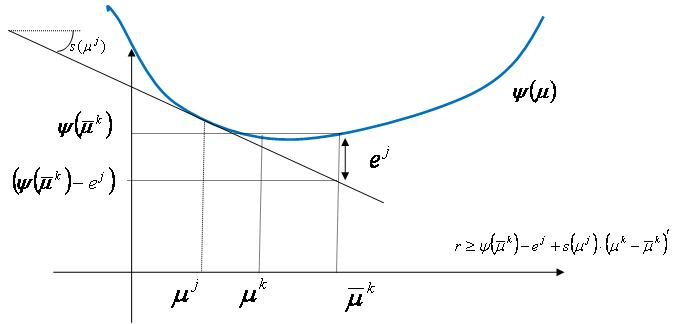
\includegraphics[width=11cm]{figuras/esquemaPBM.JPG}
	\end{center}
\end{frame}


\subsection{Ejemplo ilustrativo}

\begin{frame}
	\frametitle{Ejemplo $f(x)=3-x+\frac{x^2}{6}$: Inicialización}
	\structure{\textbf{Subgradiente asociado a $\overline{x}^0=0$}}
	\begin{center}
		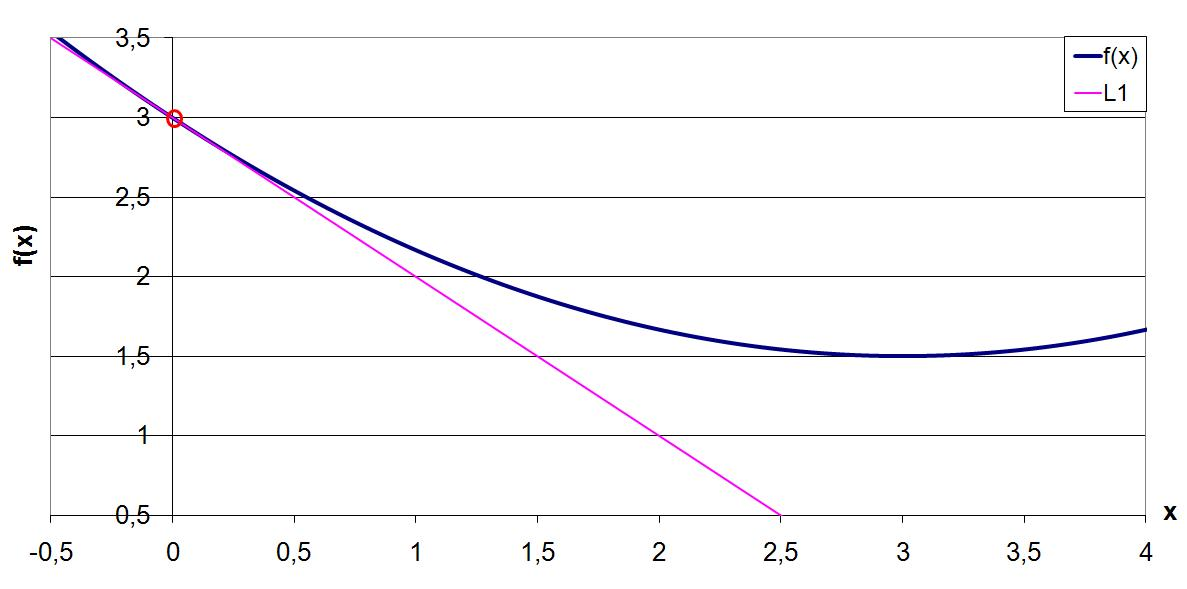
\includegraphics[width=11cm]{figuras/ejemplo01.JPG}
	\end{center}
\end{frame}

\begin{frame}
	\frametitle{Ejemplo $f(x)=3-x+\frac{x^2}{6}$: Iteración 1}
	\structure{\textbf{Función cuadrática asociada a $x^1 \rightarrow \overline{x}^1=2$}}
	\begin{center}
		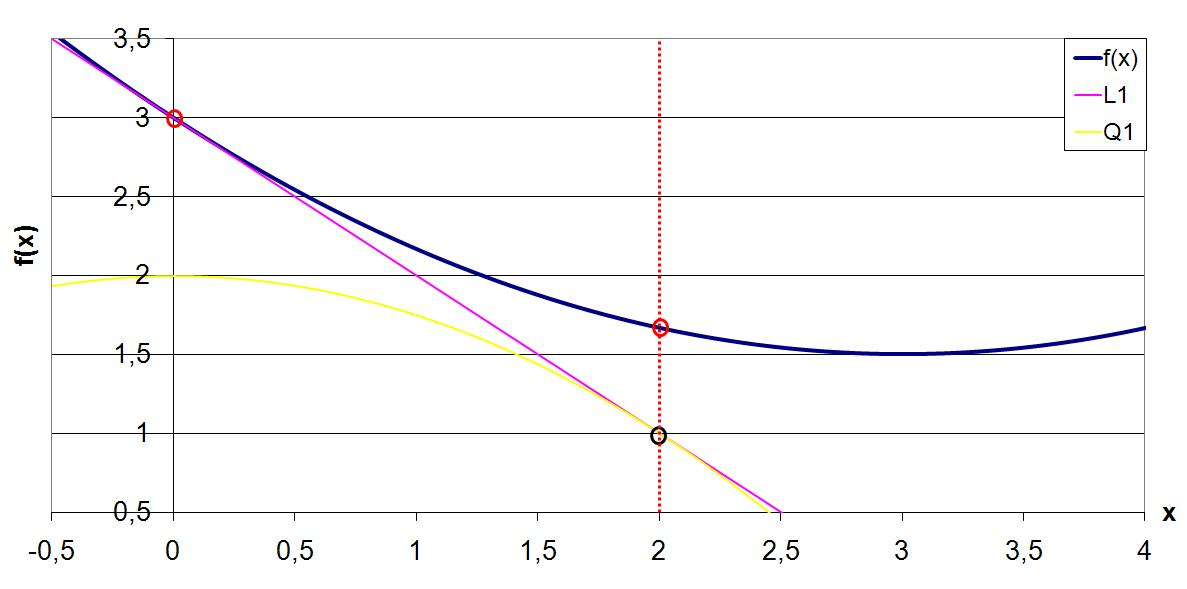
\includegraphics[width=11cm]{figuras/ejemplo02.JPG}
	\end{center}
\end{frame}

\begin{frame}
	\frametitle{Ejemplo $f(x)=3-x+\frac{x^2}{6}$: Iteración 1}
	\structure{\textbf{Subgradiente asociado a $\overline{x}^1$}}
	\begin{center}
		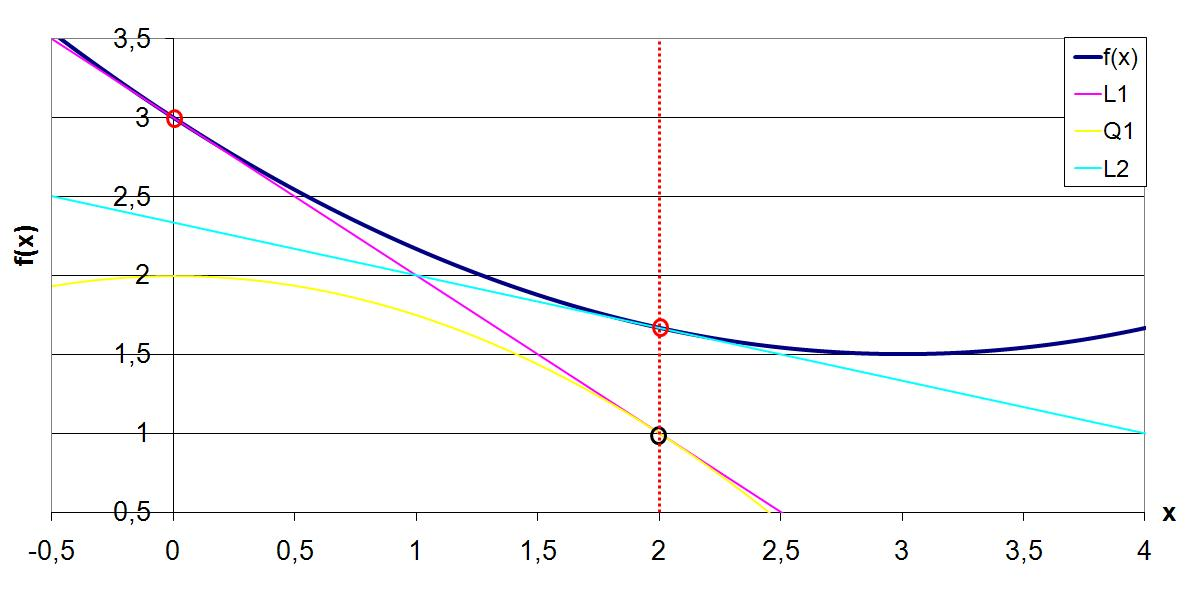
\includegraphics[width=11cm]{figuras/ejemplo03.JPG}
	\end{center}
\end{frame}

\begin{frame}
	\frametitle{Ejemplo $f(x)=3-x+\frac{x^2}{6}$: Iteración 2}
	\structure{\textbf{Función cuadrática asociada a $x^2 \rightarrow \overline{x}^2=2,\wideparen{3}$}}
	\begin{center}
		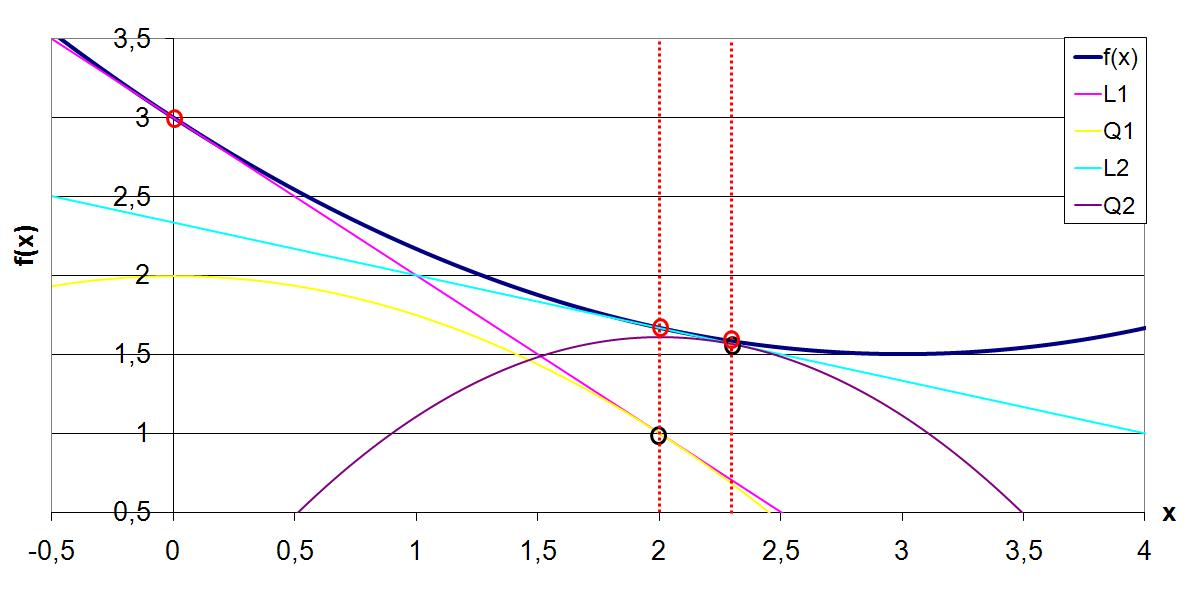
\includegraphics[width=11cm]{figuras/ejemplo04.JPG}
	\end{center}
\end{frame}

\begin{frame}
	\frametitle{Ejemplo $f(x)=3-x+\frac{x^2}{6}$: Iteración 2}
	\structure{\textbf{Subgradiente asociado a $\overline{x}^2$}}
	\begin{center}
		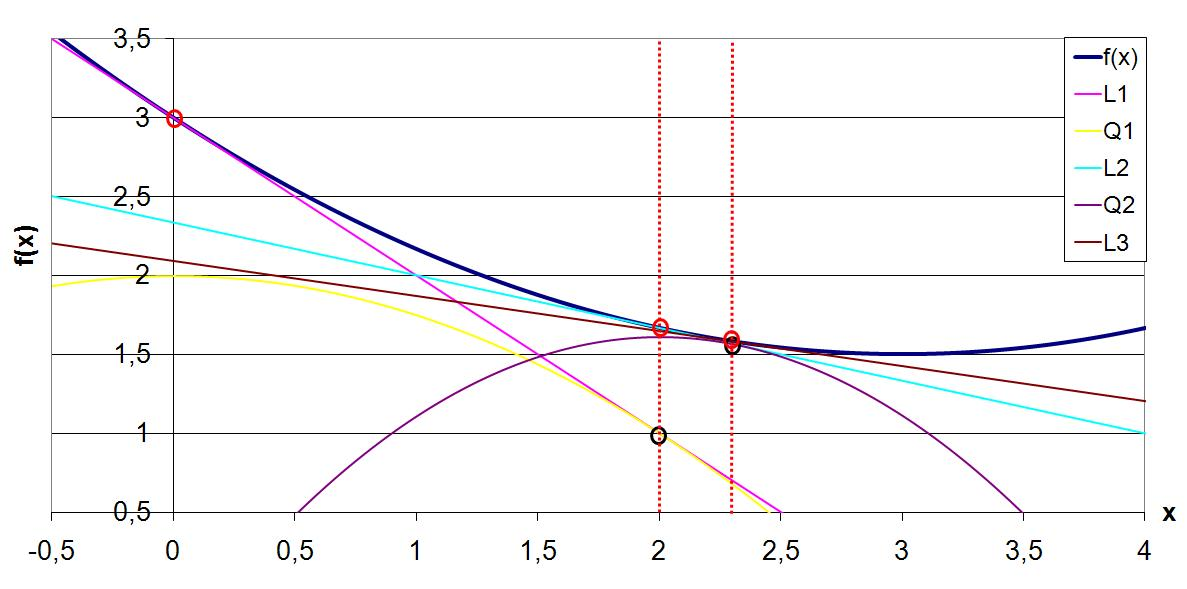
\includegraphics[width=11cm]{figuras/ejemplo05.JPG}
	\end{center}
\end{frame}

\begin{frame}
	\frametitle{Ejemplo $f(x)=3-x+\frac{x^2}{6}$: Iteración 3}
	\structure{\textbf{Función cuadrática asociada a $x^3 \rightarrow \overline{x}^3=2,\wideparen{4}$}}
	\begin{center}
		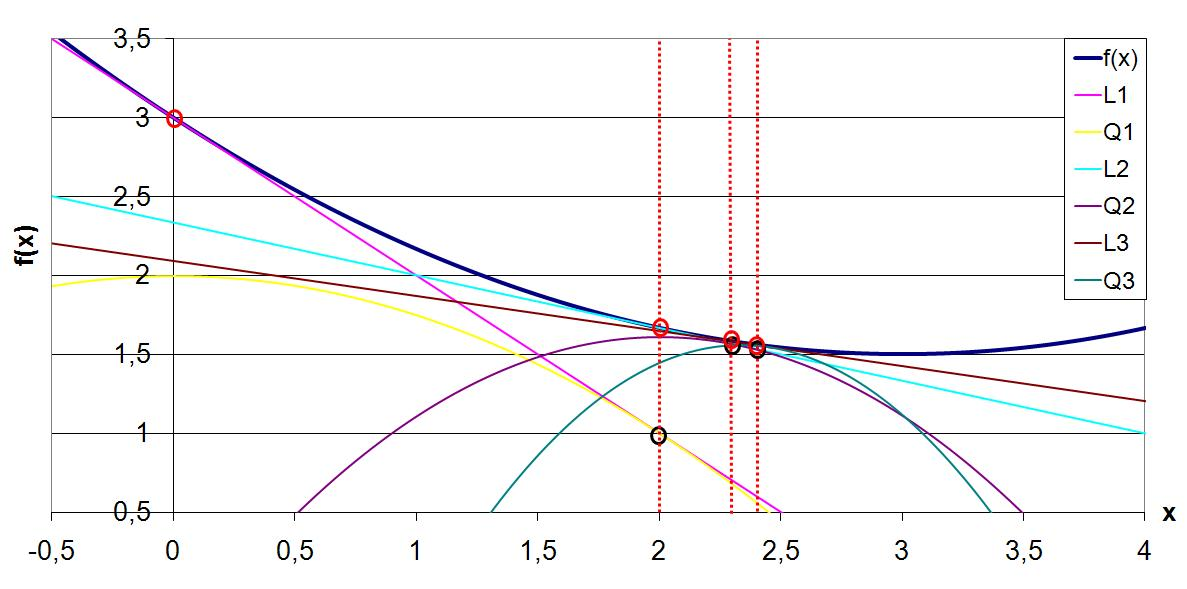
\includegraphics[width=11cm]{figuras/ejemplo06.JPG}
	\end{center}
\end{frame}

\begin{frame}
	\frametitle{Ejemplo $f(x)=3-x+\frac{x^2}{6}$: Iteración 3}
	\structure{\textbf{Subgradiente asociado a $\overline{x}^3$}}
	\begin{center}
		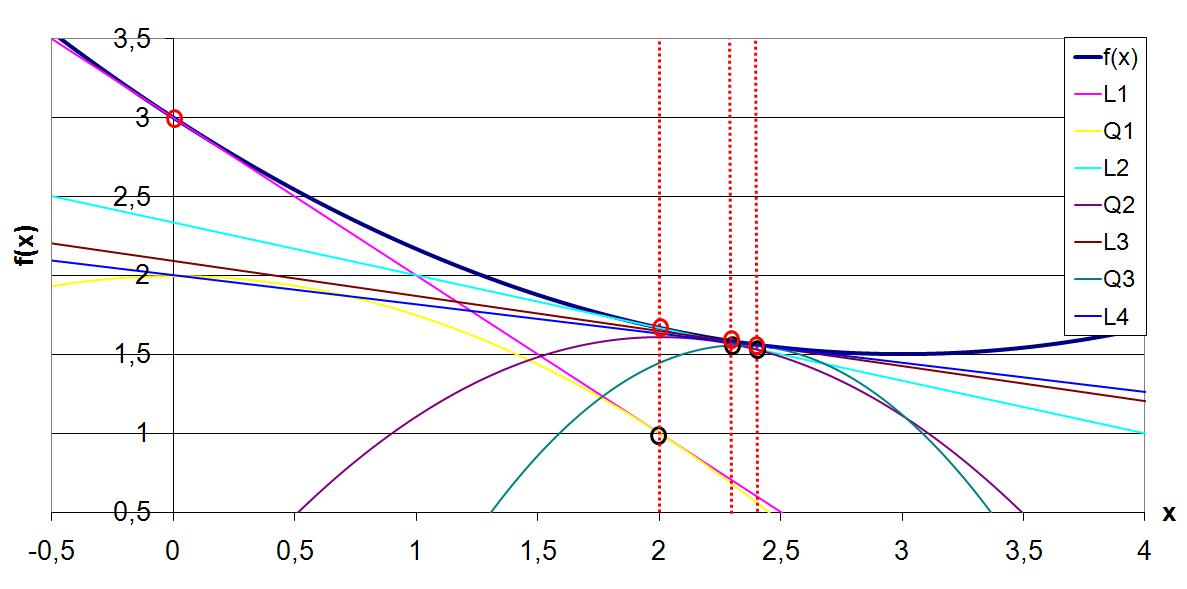
\includegraphics[width=11cm]{figuras/ejemplo07.JPG}
	\end{center}
\end{frame}


\subsection{Algoritmo Proximal Bundle Method}

\begin{frame}
	\frametitle{Algoritmo Proximal Bundle Method}
	\begingroup
	\setbeamercolor{block title}{bg=Black} %bg=background, fg= foreground
		\begin{block} {Paso 0: INICIALIZACIÓN}
			\begin{description}
				\item [Paso 0.01] Seleccionar el punto inicial $\mu_1$
				\item [Paso 0.02] Seleccionar el tamaño máximo del Bundle $\overline{\beta}$
				\item [Paso 0.06] Fijar el número máximo de iteraciones $K_{max}$
				\item [Paso 0.03] Inicializar el contador de iteraciones $k = 1$
				\item [Paso 0.04] Inicializar el tamaño del Bundle $\beta = 1$
				\item [Paso 0.05] Calcular $s_1 = s(\mu_1)$
				\item [Paso 0.06] Fijar $e_1 = 0$
				\item [Paso 0.07] Fijar una valor de la función objetivo de parada $\Lambda$
				\item [Paso 0.08] Seleccionar la longitud de paso inicial $t^1$
			\end{description}
		\end{block}
	\endgroup
\end{frame}


\begin{frame}
	\frametitle{Algoritmo Proximal Bundle Method}
	\begingroup
	\setbeamercolor{block title}{bg=Black} %bg=background, fg= foreground
		\begin{block} {Paso 1: COMPUTACIÓN PRINCIPAL}
			\begin{description}
				\item [Paso 1.01] Elegir una longitud de paso $t^k > 0$
				\item [Paso 1.02] Resolver el problema de optimización \eqref{eq:subpr}
			\end{description}
		\end{block}
		\begin{block} {Paso 2: TEST DE DESCENSO}
			\begin{description}
				\item [Paso 2.01] Calcular $\Psi(\mu^{k+1})$ y $s(\mu^{k+1})$
				\item [Paso 2.02] Si $\Psi(\mu^{k+1}) \leq \Lambda$ \textbf{STOP} \\
				\item [Paso 2.02] Si $\Psi(\mu^{k+1}) \nleq \Psi(\overline{\mu}^{k})$ \\
				Paso: NULO $\rightarrow$ Ir a \textbf{Paso 4}
			\end{description}
		\end{block}
	\endgroup
\end{frame}

\begin{frame}
	\frametitle{Algoritmo Proximal Bundle Method}
	\begingroup
	\setbeamercolor{block title}{bg=Black} %bg=background, fg= foreground
		\begin{block} {Paso 3: PASO DE DESCENSO}
			\begin{description}
				\item [Paso 3.01] $\overline{\mu}^{k+1}:= \mu^{k+1}$ Paso: DESCENSO
				\item [Paso 3.02] Para $j \in \beta$ hacer \\
				$e^j := e^j + \Psi(\overline{\mu}^{k+1})-\Psi(\overline{\mu}^{k})-\langle 	s^j,\overline{\mu}^{k+1},\overline{\mu}^{k} \rangle$		
			\end{description}
		\end{block}
		\begin{block} {Paso 4: GESTIÓN DEL TAMAÑO DEL BUNDLE}
			\begin{description}
				\item [Paso 4.01] Si $\beta = \overline{\beta}$ entonces \\
				Eliminar el elemento $(s^j,e^j) \quad j  \in \beta$ de mayor $e^j$
			\end{description}
		\end{block}
	\endgroup
\end{frame}



\begin{frame}
	\frametitle{Algoritmo Proximal Bundle Method}
	\begingroup
	\setbeamercolor{block title}{bg=Black} %bg=background, fg= foreground
		\begin{block} {Paso 5: ADICIÓN DEL NUEVO ELEMENTO AL BUNDLE}
			\begin{description}
				\item [Paso 5.01] Insertar el elemento $(s^{j+1},e^{j+1})$ al Bundle, donde \\
				$e^{j+1}=0$ si PASO DE DESCENSO \\
				$e^{j+1}=\Psi(\overline{\mu}^{k})-[\Psi({\mu}^{k+1})+\langle 	s^{j+1},\overline{\mu}^{k},\overline{\mu}^{k+1} \rangle]$ si PASO DE NULO		
				\item [Paso 5.02] Remplazar $k$ por $k+1$ e ir al PASO 1
			\end{description}
		\end{block}
	\endgroup
\end{frame}

\section{Adaptación del problema al PBM}

\begin{frame}
	\frametitle{Formulación de la función dual Lagrangiana}
	\begingroup
	\setbeamercolor{block title}{bg=NavyBlue} %bg=background, fg= foreground
		\begin{block} {PROBLEMA ORIGINAL}
			\begin{align}
				\max_{p,q,f,b} \sum_{t \in T} \sum_{i \in I} \Big\{-c^{u}_{it}-c^{d}_{it}-c^{b}_{i}u_{it}+\sum_{s\in S}P^s \Big[ \lambda^{D,s}_t p^{M,s}_{it}+ \nonumber\\
				\lambda^{R,s}_t r^{s}_{it} g_i + \lambda^{I,s}_t w^{s}_{it}-\Big( c^l_i p^s_{it} + c^q_i ( p^s_{it})^2 \Big) \Big] \Big\}= \nonumber\\		
				\max_{p,q,f,b} \sum_{t \in T} \sum_{i \in I} C(p,q,f,b) \nonumber \quad \quad \eqref{eq:Fobj}
			\end{align}
			\begin{displaymath}
				\text{s.a} \quad \eqref{eq:Fini}, \eqref{eq:Ffin}, \tau_i \quad \forall i \in I
			\end{displaymath}
		\end{block}
	\endgroup
\end{frame}


\begin{frame}
	\frametitle{Formulación de la función dual Lagrangiana}
	\begingroup
	\setbeamercolor{block title}{bg=NavyBlue} %bg=background, fg= foreground
		\begin{block} {TRANSFORMACIÓN A PROBLEMA DE MINIMIZACIÓN}
			\begin{align}
				\min_{p,q,f,b} \sum_{t \in T} \sum_{i \in I} -C(p,q,f,b)
			\end{align}
			\begin{displaymath}
				\text{s.a} \quad \eqref{eq:Fini}, \eqref{eq:Ffin}, \tau_i \quad \forall i \in I
			\end{displaymath}
		\end{block}
	\endgroup
\end{frame}


\begin{frame}
	\frametitle{Formulación de la función dual Lagrangiana}
	\begingroup
	\setbeamercolor{block title}{bg=NavyBlue} %bg=background, fg= foreground
		\begin{block} {RELAJACIÓN LAGRANGIANA}
			\begin{align}
				\phi(\mu^F,\mu^B)=\min_{p,q,f,b} \sum_{t \in T} \sum_{j \in F} \mu_{t,j}^F \Big( L_j^{FC}-\sum_{i \in U_j}f_{itj} \Big)   \nonumber \\	
				+ \sum_{t \in T} \mu_{t}^B \Big( \sum_{bc \in BC} L_{bc,t}^{BC}-\sum_{i \in I} b_{it} \Big) +\sum_{t \in T} \sum_{i \in I}-C(p,q,f,b) 
			\end{align}
			\begin{displaymath}
				\text{s.a} \quad \tau_i \quad \forall i \in I
			\end{displaymath}
		\end{block}
	\endgroup
	\textbf{cambio de notación}
	\begin{displaymath}
		\sum_{i \in U_j}f_{itj} =   \sum_{i \in I}f_{itj}J_{ij}
	\end{displaymath}
\end{frame}


\begin{frame}
	\frametitle{Formulación de la función dual Lagrangiana}
	\begingroup
	\setbeamercolor{block title}{bg=NavyBlue} %bg=background, fg= foreground
		\begin{block} {RELAJACIÓN LAGRANGIANA}
			\begin{align}
			\phi(\mu^F,\mu^B)=\min_{p,q,f,b} \sum_{t \in T} \sum_{i \in I} \Big\{ -C(p,q,f,b)- \sum_{j \in F} 	\mu_{t,j}^F  f_{itj}J_{ij} \nonumber \\		
			- \mu_{t}^{B} b_{it} \Big\} \sum_{t \in T} \sum_{j \in F} \mu^{F}_{t,j} L^{FC}_{j}+	\sum_{t \in T} \sum_{bc \in BC} \mu^{B}_{t} L^{BC}_{bc,t}
			\end{align}
			\begin{displaymath}
				\text{s.a} \quad \tau_i \quad \forall i \in I
			\end{displaymath}
		\end{block}
	\endgroup
\end{frame}


\begin{frame}
	\frametitle{Formulación de la función dual Lagrangiana}
	\begingroup
	\setbeamercolor{block title}{bg=NavyBlue} %bg=background, fg= foreground
		\begin{block} {DIVISIÓN EN SUBPROBLEMAS}
			\begin{align}
				\phi(\mu^F,\mu^B)= \sum_{i \in I} \phi_i (\mu^F,\mu^B)
				+ \sum_{t \in T} \Big( \sum_{j \in F} \mu^{F}_{t,j} L^{FC}_{j}+ \sum_{bc \in BC} \mu^{B}_{t} L^{BC}_{bc,t}  \Big)	
			\end{align}
			\begin{displaymath}
				\text{s.a} \quad \tau_i \quad \forall i \in I
			\end{displaymath}
		\end{block}
	\endgroup
	\textbf{donde}
	\begin{displaymath}
		\phi_i (\mu^F,\mu^B)= \sum_{t \in T} \Big\{ -C(p,q,f,b)- \sum_{j \in F} \mu_{t,j}^F  f_{itj}J_{ij} - 	\mu_{t}^{B} b_{it} \Big\}	
	\end{displaymath}
\end{frame}


\begin{frame}
	\frametitle{Formulación de la función dual Lagrangiana}
	\begingroup
	\setbeamercolor{block title}{bg=NavyBlue} %bg=background, fg= foreground
		\begin{block} {FUNCIÓN DUAL LAGRANGIANA}
			\begin{align}
				L^{*}=\max \phi(\mu^F,\mu^B)	
			\end{align}
			\begin{displaymath}
				\text{s.a} \quad \mu^F,\mu^B \quad \text{libres}
			\end{displaymath}
		\end{block}
	\endgroup
\end{frame}


\section {Implementación}

\begin{frame}
	\frametitle{C++ \& CPLEX: Paradigma Callable Library}
	\begin{center}
		\xymatrix@R=1.5cm @C=3cm{
		&*+[F] \txt{User-Written Application} \ar[d] \\
		&*+[F] \txt{CPLEX Callable Library} \ar[u] \ar[d] \\
		&*+[F] \txt{CPLEX internals} \ar[u]		
		}
	\end{center}
\end{frame}

\begin{frame}
	\frametitle{C++ \& CPLEX: Paradigma Concert Technology}
	\begin{center}
		\xymatrix@R=1.5cm @C=0.2cm{
		&*{} &*+[F] \txt{User-Written Application} \ar[dl] \ar[dr] \\
		&*+[F] \txt{Concert Techology \\ modeling objects} \ar[ur] 
		&*{} \ar[l] \ar[r] &*+[F] \txt{IloCplex object \\ \\ \\ CPLEX internals} \ar[ul] 
		}
	\end{center}
\end{frame}


\section {Resultados}

\begin{frame}
	\frametitle{Condiciones de resolución}
	\begin{exampleblock} {Equipo informático}
		Procesador de un solo núcleo, función de costes lineal
	\end{exampleblock}
	\begin{exampleblock} {Dimensiones del problema}
		\begin{itemize}
			\begin{columns}
				\begin{column} {.40\textwidth}
					\item $|I|=10$
					\item $|T|=24$
					\item $|S|=25$
				\end{column}
				\begin{column} {.40\textwidth}
					\item $N_{restricciones}=47040$
					\item $N_{var-lin}=19680$
					\item $N_{var-bin}=6240$
				\end{column}
			\end{columns}
		\end{itemize}
	\end{exampleblock}
\end{frame}


\subsection{Resumen de resultados}

\begin{frame}
	\frametitle{Resumen de resultados obtenidos}
	\begin{center}
		\begin{tabular}{p{3.5cm}p{2cm}p{2cm}p{2.2cm}}
			\toprule
			\textbf{Tamaño de Bundle} & \textbf{Iteraciones realizadas} & \textbf{Tiempo de ejecución} & \textbf{Tiempo por iteración} \\
			\midrule
			5 pares de elementos & 155 & 21100 & 136,13 \\
			10 pares de elementos & 143 & 21824 & 152,62 \\
% 			\hline
			20 pares de elementos & 116 & 14538 & 125,33 \\
% 			\hline
			30 pares de elementos & 76 & 7698 & 101,29 \\
% 			\hline
			Ilimitado & 62 & 5535 & 89,27 \\
% 			\hline
% 			& & & \\
% 			\hline
			\midrule
			\textbf{SUBGRADIENTE} & 300 & 19810 & 66,03 \\
			\bottomrule
		\end{tabular}
	\end{center}
\end{frame}


\subsection{Resultados iterativos}

\begin{frame}
	\frametitle{Comparación de resultados iterativos}
	\begin{center}
		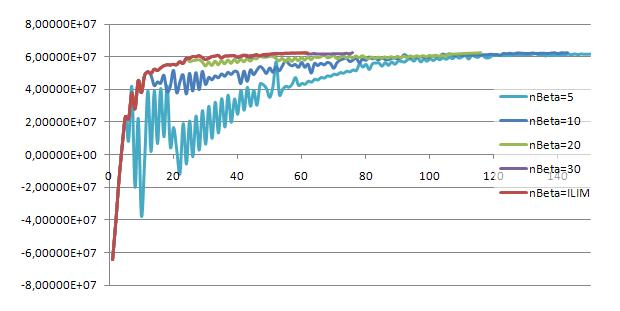
\includegraphics[width=10cm]{figuras/procesoIterativo.JPG}
	\end{center}
\end{frame}

\begin{frame}
	\frametitle{Comparación de resultados iterativos (Zoom)}
	\begin{center}
		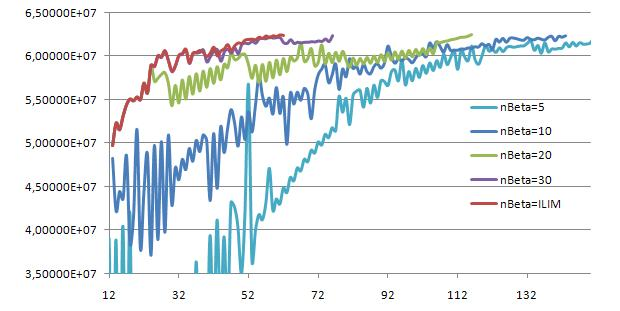
\includegraphics[width=10cm]{figuras/procesoIterativoZoom.JPG}
	\end{center}
\end{frame}

\section{Conclusiones y líneas futuras}

\begin{frame}
	\frametitle{Conclusiones}
	\begin{itemize}
		\item Se han aportado mejoras al modelo
		\item Implementación satisfactoria de PBM
		\item Desigual valoración de Concert Technology
		\item Tiempo de ejecución significativamente inferior al método del subgradiente
		\item Mejores resultados obtenidos: tamaño ilimitado de Bundle
	\end{itemize}
\end{frame}

\begin{frame}
	\frametitle{Líneas futuras}
	\begin{itemize}
		\item Programación en paralelo mediante \textbf{OpenMP} o \textbf{MPI}
		\item \textbf{Método heurístico} de recuperación de factibilidad
		\item Definir el subproblema asociado a cada unidad como un problema de \textbf{caminos mínimos}
		\item Mejora del \textbf{criterio de eliminación} de elementos
	\end{itemize}
\end{frame}



\end{document}